% Generated by Sphinx.
\def\sphinxdocclass{report}
\documentclass[letterpaper,10pt,english]{sphinxmanual}
\usepackage[utf8]{inputenc}
\DeclareUnicodeCharacter{00A0}{\nobreakspace}
\usepackage{cmap}
\usepackage[T1]{fontenc}
\usepackage{babel}
\usepackage{times}
\usepackage[Bjarne]{fncychap}
\usepackage{longtable}
\usepackage{sphinx}
\usepackage{multirow}


\title{pynoddy Documentation}
\date{March 29, 2014}
\release{}
\author{Florian Wellmann}
\newcommand{\sphinxlogo}{}
\renewcommand{\releasename}{Release}
\makeindex

\makeatletter
\def\PYG@reset{\let\PYG@it=\relax \let\PYG@bf=\relax%
    \let\PYG@ul=\relax \let\PYG@tc=\relax%
    \let\PYG@bc=\relax \let\PYG@ff=\relax}
\def\PYG@tok#1{\csname PYG@tok@#1\endcsname}
\def\PYG@toks#1+{\ifx\relax#1\empty\else%
    \PYG@tok{#1}\expandafter\PYG@toks\fi}
\def\PYG@do#1{\PYG@bc{\PYG@tc{\PYG@ul{%
    \PYG@it{\PYG@bf{\PYG@ff{#1}}}}}}}
\def\PYG#1#2{\PYG@reset\PYG@toks#1+\relax+\PYG@do{#2}}

\expandafter\def\csname PYG@tok@gd\endcsname{\def\PYG@tc##1{\textcolor[rgb]{0.63,0.00,0.00}{##1}}}
\expandafter\def\csname PYG@tok@gu\endcsname{\let\PYG@bf=\textbf\def\PYG@tc##1{\textcolor[rgb]{0.50,0.00,0.50}{##1}}}
\expandafter\def\csname PYG@tok@gt\endcsname{\def\PYG@tc##1{\textcolor[rgb]{0.00,0.27,0.87}{##1}}}
\expandafter\def\csname PYG@tok@gs\endcsname{\let\PYG@bf=\textbf}
\expandafter\def\csname PYG@tok@gr\endcsname{\def\PYG@tc##1{\textcolor[rgb]{1.00,0.00,0.00}{##1}}}
\expandafter\def\csname PYG@tok@cm\endcsname{\let\PYG@it=\textit\def\PYG@tc##1{\textcolor[rgb]{0.25,0.50,0.56}{##1}}}
\expandafter\def\csname PYG@tok@vg\endcsname{\def\PYG@tc##1{\textcolor[rgb]{0.73,0.38,0.84}{##1}}}
\expandafter\def\csname PYG@tok@m\endcsname{\def\PYG@tc##1{\textcolor[rgb]{0.13,0.50,0.31}{##1}}}
\expandafter\def\csname PYG@tok@mh\endcsname{\def\PYG@tc##1{\textcolor[rgb]{0.13,0.50,0.31}{##1}}}
\expandafter\def\csname PYG@tok@cs\endcsname{\def\PYG@tc##1{\textcolor[rgb]{0.25,0.50,0.56}{##1}}\def\PYG@bc##1{\setlength{\fboxsep}{0pt}\colorbox[rgb]{1.00,0.94,0.94}{\strut ##1}}}
\expandafter\def\csname PYG@tok@ge\endcsname{\let\PYG@it=\textit}
\expandafter\def\csname PYG@tok@vc\endcsname{\def\PYG@tc##1{\textcolor[rgb]{0.73,0.38,0.84}{##1}}}
\expandafter\def\csname PYG@tok@il\endcsname{\def\PYG@tc##1{\textcolor[rgb]{0.13,0.50,0.31}{##1}}}
\expandafter\def\csname PYG@tok@go\endcsname{\def\PYG@tc##1{\textcolor[rgb]{0.20,0.20,0.20}{##1}}}
\expandafter\def\csname PYG@tok@cp\endcsname{\def\PYG@tc##1{\textcolor[rgb]{0.00,0.44,0.13}{##1}}}
\expandafter\def\csname PYG@tok@gi\endcsname{\def\PYG@tc##1{\textcolor[rgb]{0.00,0.63,0.00}{##1}}}
\expandafter\def\csname PYG@tok@gh\endcsname{\let\PYG@bf=\textbf\def\PYG@tc##1{\textcolor[rgb]{0.00,0.00,0.50}{##1}}}
\expandafter\def\csname PYG@tok@ni\endcsname{\let\PYG@bf=\textbf\def\PYG@tc##1{\textcolor[rgb]{0.84,0.33,0.22}{##1}}}
\expandafter\def\csname PYG@tok@nl\endcsname{\let\PYG@bf=\textbf\def\PYG@tc##1{\textcolor[rgb]{0.00,0.13,0.44}{##1}}}
\expandafter\def\csname PYG@tok@nn\endcsname{\let\PYG@bf=\textbf\def\PYG@tc##1{\textcolor[rgb]{0.05,0.52,0.71}{##1}}}
\expandafter\def\csname PYG@tok@no\endcsname{\def\PYG@tc##1{\textcolor[rgb]{0.38,0.68,0.84}{##1}}}
\expandafter\def\csname PYG@tok@na\endcsname{\def\PYG@tc##1{\textcolor[rgb]{0.25,0.44,0.63}{##1}}}
\expandafter\def\csname PYG@tok@nb\endcsname{\def\PYG@tc##1{\textcolor[rgb]{0.00,0.44,0.13}{##1}}}
\expandafter\def\csname PYG@tok@nc\endcsname{\let\PYG@bf=\textbf\def\PYG@tc##1{\textcolor[rgb]{0.05,0.52,0.71}{##1}}}
\expandafter\def\csname PYG@tok@nd\endcsname{\let\PYG@bf=\textbf\def\PYG@tc##1{\textcolor[rgb]{0.33,0.33,0.33}{##1}}}
\expandafter\def\csname PYG@tok@ne\endcsname{\def\PYG@tc##1{\textcolor[rgb]{0.00,0.44,0.13}{##1}}}
\expandafter\def\csname PYG@tok@nf\endcsname{\def\PYG@tc##1{\textcolor[rgb]{0.02,0.16,0.49}{##1}}}
\expandafter\def\csname PYG@tok@si\endcsname{\let\PYG@it=\textit\def\PYG@tc##1{\textcolor[rgb]{0.44,0.63,0.82}{##1}}}
\expandafter\def\csname PYG@tok@s2\endcsname{\def\PYG@tc##1{\textcolor[rgb]{0.25,0.44,0.63}{##1}}}
\expandafter\def\csname PYG@tok@vi\endcsname{\def\PYG@tc##1{\textcolor[rgb]{0.73,0.38,0.84}{##1}}}
\expandafter\def\csname PYG@tok@nt\endcsname{\let\PYG@bf=\textbf\def\PYG@tc##1{\textcolor[rgb]{0.02,0.16,0.45}{##1}}}
\expandafter\def\csname PYG@tok@nv\endcsname{\def\PYG@tc##1{\textcolor[rgb]{0.73,0.38,0.84}{##1}}}
\expandafter\def\csname PYG@tok@s1\endcsname{\def\PYG@tc##1{\textcolor[rgb]{0.25,0.44,0.63}{##1}}}
\expandafter\def\csname PYG@tok@gp\endcsname{\let\PYG@bf=\textbf\def\PYG@tc##1{\textcolor[rgb]{0.78,0.36,0.04}{##1}}}
\expandafter\def\csname PYG@tok@sh\endcsname{\def\PYG@tc##1{\textcolor[rgb]{0.25,0.44,0.63}{##1}}}
\expandafter\def\csname PYG@tok@ow\endcsname{\let\PYG@bf=\textbf\def\PYG@tc##1{\textcolor[rgb]{0.00,0.44,0.13}{##1}}}
\expandafter\def\csname PYG@tok@sx\endcsname{\def\PYG@tc##1{\textcolor[rgb]{0.78,0.36,0.04}{##1}}}
\expandafter\def\csname PYG@tok@bp\endcsname{\def\PYG@tc##1{\textcolor[rgb]{0.00,0.44,0.13}{##1}}}
\expandafter\def\csname PYG@tok@c1\endcsname{\let\PYG@it=\textit\def\PYG@tc##1{\textcolor[rgb]{0.25,0.50,0.56}{##1}}}
\expandafter\def\csname PYG@tok@kc\endcsname{\let\PYG@bf=\textbf\def\PYG@tc##1{\textcolor[rgb]{0.00,0.44,0.13}{##1}}}
\expandafter\def\csname PYG@tok@c\endcsname{\let\PYG@it=\textit\def\PYG@tc##1{\textcolor[rgb]{0.25,0.50,0.56}{##1}}}
\expandafter\def\csname PYG@tok@mf\endcsname{\def\PYG@tc##1{\textcolor[rgb]{0.13,0.50,0.31}{##1}}}
\expandafter\def\csname PYG@tok@err\endcsname{\def\PYG@bc##1{\setlength{\fboxsep}{0pt}\fcolorbox[rgb]{1.00,0.00,0.00}{1,1,1}{\strut ##1}}}
\expandafter\def\csname PYG@tok@kd\endcsname{\let\PYG@bf=\textbf\def\PYG@tc##1{\textcolor[rgb]{0.00,0.44,0.13}{##1}}}
\expandafter\def\csname PYG@tok@ss\endcsname{\def\PYG@tc##1{\textcolor[rgb]{0.32,0.47,0.09}{##1}}}
\expandafter\def\csname PYG@tok@sr\endcsname{\def\PYG@tc##1{\textcolor[rgb]{0.14,0.33,0.53}{##1}}}
\expandafter\def\csname PYG@tok@mo\endcsname{\def\PYG@tc##1{\textcolor[rgb]{0.13,0.50,0.31}{##1}}}
\expandafter\def\csname PYG@tok@mi\endcsname{\def\PYG@tc##1{\textcolor[rgb]{0.13,0.50,0.31}{##1}}}
\expandafter\def\csname PYG@tok@kn\endcsname{\let\PYG@bf=\textbf\def\PYG@tc##1{\textcolor[rgb]{0.00,0.44,0.13}{##1}}}
\expandafter\def\csname PYG@tok@o\endcsname{\def\PYG@tc##1{\textcolor[rgb]{0.40,0.40,0.40}{##1}}}
\expandafter\def\csname PYG@tok@kr\endcsname{\let\PYG@bf=\textbf\def\PYG@tc##1{\textcolor[rgb]{0.00,0.44,0.13}{##1}}}
\expandafter\def\csname PYG@tok@s\endcsname{\def\PYG@tc##1{\textcolor[rgb]{0.25,0.44,0.63}{##1}}}
\expandafter\def\csname PYG@tok@kp\endcsname{\def\PYG@tc##1{\textcolor[rgb]{0.00,0.44,0.13}{##1}}}
\expandafter\def\csname PYG@tok@w\endcsname{\def\PYG@tc##1{\textcolor[rgb]{0.73,0.73,0.73}{##1}}}
\expandafter\def\csname PYG@tok@kt\endcsname{\def\PYG@tc##1{\textcolor[rgb]{0.56,0.13,0.00}{##1}}}
\expandafter\def\csname PYG@tok@sc\endcsname{\def\PYG@tc##1{\textcolor[rgb]{0.25,0.44,0.63}{##1}}}
\expandafter\def\csname PYG@tok@sb\endcsname{\def\PYG@tc##1{\textcolor[rgb]{0.25,0.44,0.63}{##1}}}
\expandafter\def\csname PYG@tok@k\endcsname{\let\PYG@bf=\textbf\def\PYG@tc##1{\textcolor[rgb]{0.00,0.44,0.13}{##1}}}
\expandafter\def\csname PYG@tok@se\endcsname{\let\PYG@bf=\textbf\def\PYG@tc##1{\textcolor[rgb]{0.25,0.44,0.63}{##1}}}
\expandafter\def\csname PYG@tok@sd\endcsname{\let\PYG@it=\textit\def\PYG@tc##1{\textcolor[rgb]{0.25,0.44,0.63}{##1}}}

\def\PYGZbs{\char`\\}
\def\PYGZus{\char`\_}
\def\PYGZob{\char`\{}
\def\PYGZcb{\char`\}}
\def\PYGZca{\char`\^}
\def\PYGZam{\char`\&}
\def\PYGZlt{\char`\<}
\def\PYGZgt{\char`\>}
\def\PYGZsh{\char`\#}
\def\PYGZpc{\char`\%}
\def\PYGZdl{\char`\$}
\def\PYGZhy{\char`\-}
\def\PYGZsq{\char`\'}
\def\PYGZdq{\char`\"}
\def\PYGZti{\char`\~}
% for compatibility with earlier versions
\def\PYGZat{@}
\def\PYGZlb{[}
\def\PYGZrb{]}
\makeatother

\begin{document}

\maketitle
\tableofcontents
\phantomsection\label{index::doc}


Contents:


\chapter{pynoddy}
\label{readme:welcome-to-pynoddy-s-documentation}\label{readme::doc}\label{readme:pynoddy}
pynoddy is a python package to write, change, and analyse kinematic
geological modelling simulations performed with Noddy (see below for
more infomration on Noddy).


\section{How does it work?}
\label{readme:how-does-it-work}
At this stage, pynoddy provides wrapper modules for existing Noddy
history (.his) and result files (.g00, etc.). It is


\section{Installation}
\label{readme:installation}
To install pynoddy simply run:

\begin{Verbatim}[commandchars=\\\{\}]
python setup.py install
\end{Verbatim}

Note:
\begin{itemize}
\item {} 
sufficient priviledges are required (i.e. run in sudo with MacOSX/
Linux and set permissions on Windows)

\end{itemize}

Important: the Noddy executable has to be in a directory defined in the
PATH variable!!


\section{Documentation}
\label{readme:documentation}

\section{Tutorial}
\label{readme:tutorial}
A tutorial starting with simple examples for changing the geological
history and visualisation of output, as well as the implementation of
stochastic simulations and uncertainty visualisation are available as
interactive ipython notebooks.

These notebooks are also included in this documentation as
non-interactive versions.


\section{Dependencies}
\label{readme:dependencies}
pynoddy depends on several standard Python packages that should be
shipped with any standard distribution (and are easy to install,
otherwise):
\begin{itemize}
\item {} 
numpy

\item {} 
matplotlib

\item {} 
pickle

\end{itemize}

The uncertainty anaysis, quantification, and visualisation methods based
on information theory are implemented in the python package pygeoinfo.
This package is available on github and part of the python package
index. It is automatically installed with the setup script provided with
this package. For more information, please see:

(todo: include package info!)

In addition, to export model results for full 3-D visualisation with
VTK, the pyevtk package is used, available on bitbucket:

\href{https://bitbucket.org/pauloh/pyevtk/src/9c19e3a54d1e?at=v0.1.0}{https://bitbucket.org/pauloh/pyevtk/src/9c19e3a54d1e?at=v0.1.0}


\section{License}
\label{readme:license}
pynoddy is free software and published under a MIT license (see license
file included in the repository). Please attribute the work when you use
it, feel free to change and adapt it otherwise!


\section{What is Noddy?}
\label{readme:what-is-noddy}
Noddy itself is a kinematic modelling program written by Mark Jessell
{[}1{]} to simulate the effect of subsequent geological events (folding,
unconformities, faulting, etc.) on a primary sedimentary pile. A typical
example would be:
\begin{enumerate}
\item {} 
Create a sedimentary pile with defined thicknesses for multiple
formations

\item {} 
Add a folding event (for example simple sinoidal folding, but complex
methods are possible!)

\item {} 
Add an unconformity and, above it, a new sedimentary pile

\item {} 
Finally, add a sequence of late faults affecting the entire system.

\end{enumerate}

The result could look something like this:
\begin{figure}[htbp]
\centering

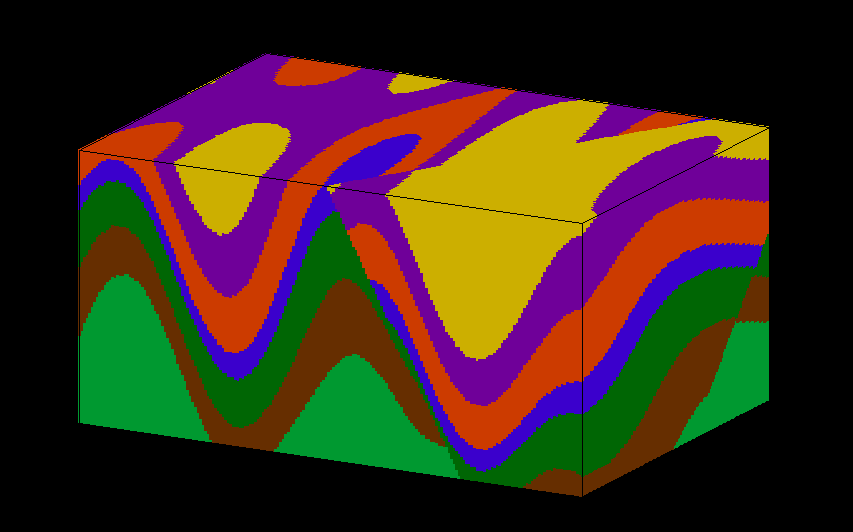
\includegraphics{noddy_block_example.png}
\end{figure}

The software runs on Windows only, but the source files (written in C)
are available for download to generate a command line version of the
modelling step alone:

\href{https://github.com/markjessell/functionNoddy}{https://github.com/markjessell/functionNoddy}

It has been tested and compiled on MacOSX, Windows and Linux.


\section{References}
\label{readme:references}
{[}1{]} Mark W. Jessell, Rick K. Valenta, Structural geophysics: Integrated
structural and geophysical modelling, In: Declan G. De Paor, Editor(s),
Computer Methods in the Geosciences, Pergamon, 1996, Volume 15, Pages
303-324, ISSN 1874-561X, ISBN 9780080424309,
\href{http://dx.doi.org/10.1016/S1874-561X(96)80027-7}{http://dx.doi.org/10.1016/S1874-561X(96)80027-7}.


\chapter{Simulation of a Noddy history and visualisation of output}
\label{notebooks/1-Simulation:simulation-of-a-noddy-history-and-visualisation-of-output}\label{notebooks/1-Simulation::doc}
Examples of how the module can be used to run Noddy simulations and
visualise the output.

\begin{Verbatim}[commandchars=\\\{\}]
\PYG{c}{\PYGZsh{} Basic settings}
\PYG{k+kn}{import} \PYG{n+nn}{sys}\PYG{o}{,} \PYG{n+nn}{os}
\PYG{k+kn}{import} \PYG{n+nn}{subprocess}

\PYG{c}{\PYGZsh{} Now import pynoddy}
\PYG{k+kn}{import} \PYG{n+nn}{pynoddy}

\PYG{c}{\PYGZsh{} determine path of repository to set paths corretly below}

\PYG{n}{repo\PYGZus{}path} \PYG{o}{=} \PYG{n}{os}\PYG{o}{.}\PYG{n}{path}\PYG{o}{.}\PYG{n}{realpath}\PYG{p}{(}\PYG{l+s}{\PYGZsq{}}\PYG{l+s}{../..}\PYG{l+s}{\PYGZsq{}}\PYG{p}{)}
\end{Verbatim}


\section{(1) Compute the model}
\label{notebooks/1-Simulation:compute-the-model}
The simplest way to perform the Noddy simulation through Python is
simply to call the executable. One way that should be fairly platform
independent is to use Python's own subprocess module:

\begin{Verbatim}[commandchars=\\\{\}]
\PYG{c}{\PYGZsh{} Change to sandbox directory to store results}
\PYG{n}{os}\PYG{o}{.}\PYG{n}{chdir}\PYG{p}{(}\PYG{n}{os}\PYG{o}{.}\PYG{n}{path}\PYG{o}{.}\PYG{n}{join}\PYG{p}{(}\PYG{n}{repo\PYGZus{}path}\PYG{p}{,} \PYG{l+s}{\PYGZsq{}}\PYG{l+s}{sandbox}\PYG{l+s}{\PYGZsq{}}\PYG{p}{)}\PYG{p}{)}

\PYG{c}{\PYGZsh{} Path to exmaple directory in this repository}
\PYG{n}{example\PYGZus{}directory} \PYG{o}{=} \PYG{n}{os}\PYG{o}{.}\PYG{n}{path}\PYG{o}{.}\PYG{n}{join}\PYG{p}{(}\PYG{n}{repo\PYGZus{}path}\PYG{p}{,}\PYG{l+s}{\PYGZsq{}}\PYG{l+s}{examples}\PYG{l+s}{\PYGZsq{}}\PYG{p}{)}
\PYG{c}{\PYGZsh{} Compute noddy model for history file}
\PYG{n}{history\PYGZus{}file} \PYG{o}{=} \PYG{l+s}{\PYGZsq{}}\PYG{l+s}{simple\PYGZus{}two\PYGZus{}faults.his}\PYG{l+s}{\PYGZsq{}}
\PYG{n}{history} \PYG{o}{=} \PYG{n}{os}\PYG{o}{.}\PYG{n}{path}\PYG{o}{.}\PYG{n}{join}\PYG{p}{(}\PYG{n}{example\PYGZus{}directory}\PYG{p}{,} \PYG{n}{history\PYGZus{}file}\PYG{p}{)}
\PYG{n}{output\PYGZus{}name} \PYG{o}{=} \PYG{l+s}{\PYGZsq{}}\PYG{l+s}{noddy\PYGZus{}out}\PYG{l+s}{\PYGZsq{}}
\PYG{c}{\PYGZsh{} call Noddy}

\PYG{c}{\PYGZsh{} NOTE: Make sure that the noddy executable is accessible in the system!!}
\PYG{n}{sys}
\PYG{k}{print} \PYG{n}{subprocess}\PYG{o}{.}\PYG{n}{Popen}\PYG{p}{(}\PYG{p}{[}\PYG{l+s}{\PYGZsq{}}\PYG{l+s}{noddy}\PYG{l+s}{\PYGZsq{}}\PYG{p}{,} \PYG{n}{history}\PYG{p}{,} \PYG{n}{output\PYGZus{}name}\PYG{p}{]}\PYG{p}{,}
                       \PYG{n}{shell}\PYG{o}{=}\PYG{n+nb+bp}{False}\PYG{p}{,} \PYG{n}{stderr}\PYG{o}{=}\PYG{n}{subprocess}\PYG{o}{.}\PYG{n}{PIPE}\PYG{p}{,}
                       \PYG{n}{stdout}\PYG{o}{=}\PYG{n}{subprocess}\PYG{o}{.}\PYG{n}{PIPE}\PYG{p}{)}\PYG{o}{.}\PYG{n}{stdout}\PYG{o}{.}\PYG{n}{read}\PYG{p}{(}\PYG{p}{)}
\PYG{c}{\PYGZsh{}}
\end{Verbatim}

For convenience, the model computation is wrapped into a Python function
in pynoddy:

\begin{Verbatim}[commandchars=\\\{\}]
\PYG{n}{pynoddy}\PYG{o}{.}\PYG{n}{compute\PYGZus{}model}\PYG{p}{(}\PYG{n}{history}\PYG{p}{,} \PYG{n}{output\PYGZus{}name}\PYG{p}{)}
\end{Verbatim}

Note: The Noddy call from Python is, to date, calling Noddy through the
subprocess function. In a future implementation, this call could be
subsituted with a full wrapper for the C-functions written in Python.
Therefore, using the member function compute\_model is not only easier,
but also the more ``future-proof'' way to compute the Noddy model.


\section{(2) Loading Noddy output files}
\label{notebooks/1-Simulation:loading-noddy-output-files}
Noddy simulations produce a variety of different output files, depending
on the type of simulation. The basic output is the geological model.
Additional output files can contain geophysical responses, etc.

Loading the output files is simplified with a class class container that
reads all relevant information and provides simple methods for plotting,
model analysis, and export. To load the output information into a Python
object:

\begin{Verbatim}[commandchars=\\\{\}]
\PYG{n}{N1} \PYG{o}{=} \PYG{n}{pynoddy}\PYG{o}{.}\PYG{n}{NoddyOutput}\PYG{p}{(}\PYG{n}{output\PYGZus{}name}\PYG{p}{)}
\end{Verbatim}

The object contains the calculated geology blocks and some additional
information on grid spacing, model extent, etc. For example:

\begin{Verbatim}[commandchars=\\\{\}]
\PYG{k}{print}\PYG{p}{(}\PYG{l+s}{\PYGZdq{}}\PYG{l+s}{The model has an extent of }\PYG{l+s+si}{\PYGZpc{}.0f}\PYG{l+s}{ m in x\PYGZhy{}direction, with }\PYG{l+s+si}{\PYGZpc{}d}\PYG{l+s}{ cells of width }\PYG{l+s+si}{\PYGZpc{}.0f}\PYG{l+s}{ m}\PYG{l+s}{\PYGZdq{}} \PYG{o}{\PYGZpc{}}
      \PYG{p}{(}\PYG{n}{N1}\PYG{o}{.}\PYG{n}{extent\PYGZus{}x}\PYG{p}{,} \PYG{n}{N1}\PYG{o}{.}\PYG{n}{nx}\PYG{p}{,} \PYG{n}{N1}\PYG{o}{.}\PYG{n}{delx}\PYG{p}{)}\PYG{p}{)}
\end{Verbatim}

\begin{Verbatim}[commandchars=\\\{\}]
The model has an extent of 12400 m in x\PYGZhy{}direction, with 62 cells of width 200 m
\end{Verbatim}


\section{(3) Plotting sections through the model}
\label{notebooks/1-Simulation:plotting-sections-through-the-model}
The NoddyOutput class has some basic methods for the visualisation of
the generated models. To plot sections through the model:

\begin{Verbatim}[commandchars=\\\{\}]
\PYG{n}{N1}\PYG{o}{.}\PYG{n}{plot\PYGZus{}section}\PYG{p}{(}\PYG{l+s}{\PYGZsq{}}\PYG{l+s}{x}\PYG{l+s}{\PYGZsq{}}\PYG{p}{,} \PYG{n}{position} \PYG{o}{=} \PYG{l+m+mi}{0}\PYG{p}{)}
\end{Verbatim}

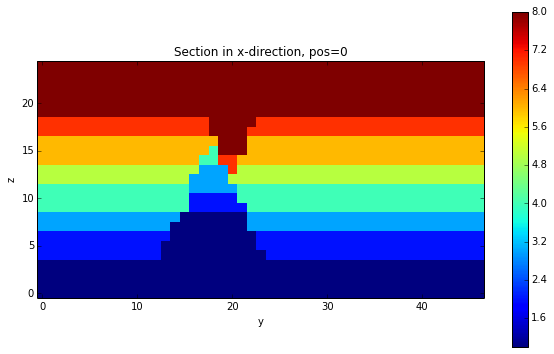
\includegraphics{1-Simulation_12_0.png}


\section{(4) Export model to VTK}
\label{notebooks/1-Simulation:export-model-to-vtk}
A simple possibility to visualise the modeled results in 3-D is to
export the model to a VTK file and then to visualise it with a VTK
viewer, for example Paraview. To export the model, simply use:

\begin{Verbatim}[commandchars=\\\{\}]
\PYG{n}{N1}\PYG{o}{.}\PYG{n}{export\PYGZus{}to\PYGZus{}vtk}\PYG{p}{(}\PYG{p}{)}
\end{Verbatim}


\chapter{Change Noddy input file and recompute model}
\label{notebooks/2-Adjust-input::doc}\label{notebooks/2-Adjust-input:change-noddy-input-file-and-recompute-model}
Visualising output of a Noddy model is nice, but not terribly helpful as
it can be done with the GUI itself. More interesting is it to change
aspects of the Noddy input (history) file with the Python module to
quickly compare the effect of changes in the geological history.

Implementing these changes in scripts is the first step to a more
extensive uncertainty analysis, as we will see in the next section.

\begin{Verbatim}[commandchars=\\\{\}]
\PYG{k+kn}{import} \PYG{n+nn}{sys}\PYG{o}{,} \PYG{n+nn}{os}
\PYG{k+kn}{import} \PYG{n+nn}{matplotlib.pyplot} \PYG{k+kn}{as} \PYG{n+nn}{plt}
\PYG{c}{\PYGZsh{} adjust some settings for matplotlib}
\PYG{k+kn}{from} \PYG{n+nn}{matplotlib} \PYG{k+kn}{import} \PYG{n}{rcParams}
\PYG{c}{\PYGZsh{} print rcParams}
\PYG{n}{rcParams}\PYG{p}{[}\PYG{l+s}{\PYGZsq{}}\PYG{l+s}{font.size}\PYG{l+s}{\PYGZsq{}}\PYG{p}{]} \PYG{o}{=} \PYG{l+m+mi}{15}
\PYG{c}{\PYGZsh{} determine path of repository to set paths corretly below}
\PYG{c}{\PYGZsh{} os.chdir(r\PYGZsq{}/Users/flow/git/pynoddy/docs/notebooks/\PYGZsq{})}
\PYG{n}{repo\PYGZus{}path} \PYG{o}{=} \PYG{n}{os}\PYG{o}{.}\PYG{n}{path}\PYG{o}{.}\PYG{n}{realpath}\PYG{p}{(}\PYG{l+s}{\PYGZsq{}}\PYG{l+s}{../..}\PYG{l+s}{\PYGZsq{}}\PYG{p}{)}
\PYG{k+kn}{import} \PYG{n+nn}{pynoddy}
\end{Verbatim}

First step: load the history file into a Python object:

\begin{Verbatim}[commandchars=\\\{\}]
\PYG{c}{\PYGZsh{} Change to sandbox directory to store results}
\PYG{n}{os}\PYG{o}{.}\PYG{n}{chdir}\PYG{p}{(}\PYG{n}{os}\PYG{o}{.}\PYG{n}{path}\PYG{o}{.}\PYG{n}{join}\PYG{p}{(}\PYG{n}{repo\PYGZus{}path}\PYG{p}{,} \PYG{l+s}{\PYGZsq{}}\PYG{l+s}{sandbox}\PYG{l+s}{\PYGZsq{}}\PYG{p}{)}\PYG{p}{)}

\PYG{c}{\PYGZsh{} Path to exmaple directory in this repository}
\PYG{n}{example\PYGZus{}directory} \PYG{o}{=} \PYG{n}{os}\PYG{o}{.}\PYG{n}{path}\PYG{o}{.}\PYG{n}{join}\PYG{p}{(}\PYG{n}{repo\PYGZus{}path}\PYG{p}{,}\PYG{l+s}{\PYGZsq{}}\PYG{l+s}{examples}\PYG{l+s}{\PYGZsq{}}\PYG{p}{)}
\PYG{c}{\PYGZsh{} Compute noddy model for history file}
\PYG{n}{history\PYGZus{}file} \PYG{o}{=} \PYG{l+s}{\PYGZsq{}}\PYG{l+s}{simple\PYGZus{}two\PYGZus{}faults.his}\PYG{l+s}{\PYGZsq{}}
\PYG{n}{history} \PYG{o}{=} \PYG{n}{os}\PYG{o}{.}\PYG{n}{path}\PYG{o}{.}\PYG{n}{join}\PYG{p}{(}\PYG{n}{example\PYGZus{}directory}\PYG{p}{,} \PYG{n}{history\PYGZus{}file}\PYG{p}{)}
\PYG{n}{output\PYGZus{}name} \PYG{o}{=} \PYG{l+s}{\PYGZsq{}}\PYG{l+s}{noddy\PYGZus{}out}\PYG{l+s}{\PYGZsq{}}
\PYG{n}{H1} \PYG{o}{=} \PYG{n}{pynoddy}\PYG{o}{.}\PYG{n}{NoddyHistory}\PYG{p}{(}\PYG{n}{history}\PYG{p}{)}
\end{Verbatim}

\begin{Verbatim}[commandchars=\\\{\}]
\PYG{l+m+mi}{8}
\end{Verbatim}


\section{(1) Get basic information on the model}
\label{notebooks/2-Adjust-input:get-basic-information-on-the-model}
The history file contains the entire information on the Noddy model.
Some information can be accessed through the NoddyHistory object (and
more will be added soon!):

\begin{Verbatim}[commandchars=\\\{\}]
\PYG{c}{\PYGZsh{} history\PYGZus{}file = \PYGZsq{}two\PYGZus{}faults\PYGZus{}fold\PYGZus{}unconformity\PYGZus{}slice.his\PYGZsq{}}
\PYG{n}{history} \PYG{o}{=} \PYG{n}{os}\PYG{o}{.}\PYG{n}{path}\PYG{o}{.}\PYG{n}{join}\PYG{p}{(}\PYG{n}{example\PYGZus{}directory}\PYG{p}{,} \PYG{n}{history\PYGZus{}file}\PYG{p}{)}
\PYG{k+kn}{import} \PYG{n+nn}{pynoddy.history}
\PYG{n+nb}{reload}\PYG{p}{(}\PYG{n}{pynoddy}\PYG{o}{.}\PYG{n}{history}\PYG{p}{)}
\PYG{n+nb}{reload}\PYG{p}{(}\PYG{n}{pynoddy}\PYG{o}{.}\PYG{n}{events}\PYG{p}{)}
\PYG{n}{H1} \PYG{o}{=} \PYG{n}{pynoddy}\PYG{o}{.}\PYG{n}{history}\PYG{o}{.}\PYG{n}{NoddyHistory}\PYG{p}{(}\PYG{n}{history}\PYG{p}{)}
\PYG{n}{H1}\PYG{o}{.}\PYG{n}{\PYGZus{}raw\PYGZus{}events}
\end{Verbatim}

\begin{Verbatim}[commandchars=\\\{\}]
\PYG{l+m+mi}{8}
\end{Verbatim}

\begin{Verbatim}[commandchars=\\\{\}]
\PYG{p}{[}\PYG{p}{\PYGZob{}}\PYG{l+s}{\PYGZsq{}}\PYG{l+s}{line\PYGZus{}end}\PYG{l+s}{\PYGZsq{}}\PYG{p}{:} \PYG{l+m+mi}{161}\PYG{p}{,} \PYG{l+s}{\PYGZsq{}}\PYG{l+s}{line\PYGZus{}start}\PYG{l+s}{\PYGZsq{}}\PYG{p}{:} \PYG{l+m+mi}{7}\PYG{p}{,} \PYG{l+s}{\PYGZsq{}}\PYG{l+s}{num}\PYG{l+s}{\PYGZsq{}}\PYG{p}{:} \PYG{l+m+mi}{1}\PYG{p}{,} \PYG{l+s}{\PYGZsq{}}\PYG{l+s}{type}\PYG{l+s}{\PYGZsq{}}\PYG{p}{:} \PYG{l+s}{\PYGZsq{}}\PYG{l+s}{ STRATIGRAPHY}\PYG{l+s}{\PYGZsq{}}\PYG{p}{\PYGZcb{}}\PYG{p}{,}
 \PYG{p}{\PYGZob{}}\PYG{l+s}{\PYGZsq{}}\PYG{l+s}{line\PYGZus{}end}\PYG{l+s}{\PYGZsq{}}\PYG{p}{:} \PYG{l+m+mi}{461}\PYG{p}{,} \PYG{l+s}{\PYGZsq{}}\PYG{l+s}{line\PYGZus{}start}\PYG{l+s}{\PYGZsq{}}\PYG{p}{:} \PYG{l+m+mi}{162}\PYG{p}{,} \PYG{l+s}{\PYGZsq{}}\PYG{l+s}{num}\PYG{l+s}{\PYGZsq{}}\PYG{p}{:} \PYG{l+m+mi}{2}\PYG{p}{,} \PYG{l+s}{\PYGZsq{}}\PYG{l+s}{type}\PYG{l+s}{\PYGZsq{}}\PYG{p}{:} \PYG{l+s}{\PYGZsq{}}\PYG{l+s}{ FAULT}\PYG{l+s}{\PYGZsq{}}\PYG{p}{\PYGZcb{}}\PYG{p}{,}
 \PYG{p}{\PYGZob{}}\PYG{l+s}{\PYGZsq{}}\PYG{l+s}{line\PYGZus{}end}\PYG{l+s}{\PYGZsq{}}\PYG{p}{:} \PYG{l+m+mi}{762}\PYG{p}{,} \PYG{l+s}{\PYGZsq{}}\PYG{l+s}{line\PYGZus{}start}\PYG{l+s}{\PYGZsq{}}\PYG{p}{:} \PYG{l+m+mi}{462}\PYG{p}{,} \PYG{l+s}{\PYGZsq{}}\PYG{l+s}{num}\PYG{l+s}{\PYGZsq{}}\PYG{p}{:} \PYG{l+m+mi}{3}\PYG{p}{,} \PYG{l+s}{\PYGZsq{}}\PYG{l+s}{type}\PYG{l+s}{\PYGZsq{}}\PYG{p}{:} \PYG{l+s}{\PYGZsq{}}\PYG{l+s}{ FAULT}\PYG{l+s}{\PYGZsq{}}\PYG{p}{\PYGZcb{}}\PYG{p}{]}
\end{Verbatim}

\begin{Verbatim}[commandchars=\\\{\}]
\PYG{n}{H1}\PYG{o}{.}\PYG{n}{events}
\end{Verbatim}

\begin{Verbatim}[commandchars=\\\{\}]
\PYGZob{}1: \PYGZlt{}pynoddy.events.Stratigraphy instance at 0x104f9b320\PYGZgt{},
 2: \PYGZlt{}pynoddy.events.Fault instance at 0x104f9b368\PYGZgt{},
 3: \PYGZlt{}pynoddy.events.Fault instance at 0x104f9b440\PYGZgt{}\PYGZcb{}
\end{Verbatim}

\begin{Verbatim}[commandchars=\\\{\}]
\PYG{n}{H1}\PYG{o}{.}\PYG{n}{events}\PYG{p}{[}\PYG{l+m+mi}{2}\PYG{p}{]}\PYG{o}{.}\PYG{n}{properties}
\PYG{c}{\PYGZsh{} print H1.events[5].properties.keys()}
\end{Verbatim}

\begin{Verbatim}[commandchars=\\\{\}]
\PYG{p}{\PYGZob{}}\PYG{l+s}{\PYGZsq{}}\PYG{l+s}{Amplitude}\PYG{l+s}{\PYGZsq{}}\PYG{p}{:} \PYG{l+m+mf}{2000.0}\PYG{p}{,}
 \PYG{l+s}{\PYGZsq{}}\PYG{l+s}{Blue}\PYG{l+s}{\PYGZsq{}}\PYG{p}{:} \PYG{l+m+mf}{254.0}\PYG{p}{,}
 \PYG{l+s}{\PYGZsq{}}\PYG{l+s}{Color Name}\PYG{l+s}{\PYGZsq{}}\PYG{p}{:} \PYG{l+s}{\PYGZsq{}}\PYG{l+s}{Custom Colour 8}\PYG{l+s}{\PYGZsq{}}\PYG{p}{,}
 \PYG{l+s}{\PYGZsq{}}\PYG{l+s}{Cyl Index}\PYG{l+s}{\PYGZsq{}}\PYG{p}{:} \PYG{l+m+mf}{0.0}\PYG{p}{,}
 \PYG{l+s}{\PYGZsq{}}\PYG{l+s}{Dip}\PYG{l+s}{\PYGZsq{}}\PYG{p}{:} \PYG{l+m+mf}{60.0}\PYG{p}{,}
 \PYG{l+s}{\PYGZsq{}}\PYG{l+s}{Dip Direction}\PYG{l+s}{\PYGZsq{}}\PYG{p}{:} \PYG{l+m+mf}{90.0}\PYG{p}{,}
 \PYG{l+s}{\PYGZsq{}}\PYG{l+s}{Event \PYGZsh{}2}\PYG{l+s}{\PYGZsq{}}\PYG{p}{:} \PYG{l+s}{\PYGZsq{}}\PYG{l+s}{FAULT}\PYG{l+s}{\PYGZsq{}}\PYG{p}{,}
 \PYG{l+s}{\PYGZsq{}}\PYG{l+s}{Geometry}\PYG{l+s}{\PYGZsq{}}\PYG{p}{:} \PYG{l+s}{\PYGZsq{}}\PYG{l+s}{Translation}\PYG{l+s}{\PYGZsq{}}\PYG{p}{,}
 \PYG{l+s}{\PYGZsq{}}\PYG{l+s}{Green}\PYG{l+s}{\PYGZsq{}}\PYG{p}{:} \PYG{l+m+mf}{0.0}\PYG{p}{,}
 \PYG{l+s}{\PYGZsq{}}\PYG{l+s}{Movement}\PYG{l+s}{\PYGZsq{}}\PYG{p}{:} \PYG{l+s}{\PYGZsq{}}\PYG{l+s}{Hanging Wall}\PYG{l+s}{\PYGZsq{}}\PYG{p}{,}
 \PYG{l+s}{\PYGZsq{}}\PYG{l+s}{Pitch}\PYG{l+s}{\PYGZsq{}}\PYG{p}{:} \PYG{l+m+mf}{90.0}\PYG{p}{,}
 \PYG{l+s}{\PYGZsq{}}\PYG{l+s}{Profile Pitch}\PYG{l+s}{\PYGZsq{}}\PYG{p}{:} \PYG{l+m+mf}{90.0}\PYG{p}{,}
 \PYG{l+s}{\PYGZsq{}}\PYG{l+s}{Radius}\PYG{l+s}{\PYGZsq{}}\PYG{p}{:} \PYG{l+m+mf}{1000.0}\PYG{p}{,}
 \PYG{l+s}{\PYGZsq{}}\PYG{l+s}{Red}\PYG{l+s}{\PYGZsq{}}\PYG{p}{:} \PYG{l+m+mf}{0.0}\PYG{p}{,}
 \PYG{l+s}{\PYGZsq{}}\PYG{l+s}{Rotation}\PYG{l+s}{\PYGZsq{}}\PYG{p}{:} \PYG{l+m+mf}{30.0}\PYG{p}{,}
 \PYG{l+s}{\PYGZsq{}}\PYG{l+s}{Slip}\PYG{l+s}{\PYGZsq{}}\PYG{p}{:} \PYG{l+m+mf}{1000.0}\PYG{p}{,}
 \PYG{l+s}{\PYGZsq{}}\PYG{l+s}{X}\PYG{l+s}{\PYGZsq{}}\PYG{p}{:} \PYG{l+m+mf}{5500.0}\PYG{p}{,}
 \PYG{l+s}{\PYGZsq{}}\PYG{l+s}{XAxis}\PYG{l+s}{\PYGZsq{}}\PYG{p}{:} \PYG{l+m+mf}{2000.0}\PYG{p}{,}
 \PYG{l+s}{\PYGZsq{}}\PYG{l+s}{Y}\PYG{l+s}{\PYGZsq{}}\PYG{p}{:} \PYG{l+m+mf}{3968.0}\PYG{p}{,}
 \PYG{l+s}{\PYGZsq{}}\PYG{l+s}{YAxis}\PYG{l+s}{\PYGZsq{}}\PYG{p}{:} \PYG{l+m+mf}{2000.0}\PYG{p}{,}
 \PYG{l+s}{\PYGZsq{}}\PYG{l+s}{Z}\PYG{l+s}{\PYGZsq{}}\PYG{p}{:} \PYG{l+m+mf}{0.0}\PYG{p}{,}
 \PYG{l+s}{\PYGZsq{}}\PYG{l+s}{ZAxis}\PYG{l+s}{\PYGZsq{}}\PYG{p}{:} \PYG{l+m+mf}{2000.0}\PYG{p}{\PYGZcb{}}
\end{Verbatim}


\section{(2) Change model cube size and recompute model}
\label{notebooks/2-Adjust-input:change-model-cube-size-and-recompute-model}
The Noddy model itself is, once computed, a continuous model in 3-D
space. However, for most visualisations and further calculations (e.g.
geophysics), a discretised version is suitable. The discretisation (or
block size) can be adapted in the history file. The according pynoddy
function is change\_cube\_size.

A simple example to change the cube size and write a new history file:

\begin{Verbatim}[commandchars=\\\{\}]
\PYG{c}{\PYGZsh{} We will first recompute the model and store results in an output file for comparison}
\PYG{n+nb}{reload}\PYG{p}{(}\PYG{n}{pynoddy}\PYG{p}{)}
\PYG{n}{NH1} \PYG{o}{=} \PYG{n}{pynoddy}\PYG{o}{.}\PYG{n}{NoddyHistory}\PYG{p}{(}\PYG{n}{history}\PYG{p}{)}
\PYG{n}{pynoddy}\PYG{o}{.}\PYG{n}{compute\PYGZus{}model}\PYG{p}{(}\PYG{n}{history}\PYG{p}{,} \PYG{n}{output\PYGZus{}name}\PYG{p}{)}
\PYG{n}{NO1} \PYG{o}{=} \PYG{n}{pynoddy}\PYG{o}{.}\PYG{n}{NoddyOutput}\PYG{p}{(}\PYG{n}{output\PYGZus{}name}\PYG{p}{)}
\end{Verbatim}

\begin{Verbatim}[commandchars=\\\{\}]
\PYG{l+m+mi}{8}
\end{Verbatim}

\begin{Verbatim}[commandchars=\\\{\}]
\PYG{c}{\PYGZsh{} Now: change cubsize, write to new file and recompute}
\PYG{n}{NH1}\PYG{o}{.}\PYG{n}{change\PYGZus{}cube\PYGZus{}size}\PYG{p}{(}\PYG{l+m+mi}{50}\PYG{p}{)}
\PYG{c}{\PYGZsh{} Save model to a new history file and recompute (Note: may take a while to compute now)}
\PYG{n}{new\PYGZus{}history} \PYG{o}{=} \PYG{l+s}{\PYGZdq{}}\PYG{l+s}{fault\PYGZus{}model\PYGZus{}changed\PYGZus{}cubesize.his}\PYG{l+s}{\PYGZdq{}}
\PYG{n}{new\PYGZus{}output\PYGZus{}name} \PYG{o}{=} \PYG{l+s}{\PYGZdq{}}\PYG{l+s}{noddy\PYGZus{}out\PYGZus{}changed\PYGZus{}cube}\PYG{l+s}{\PYGZdq{}}
\PYG{n}{NH1}\PYG{o}{.}\PYG{n}{write\PYGZus{}history}\PYG{p}{(}\PYG{n}{new\PYGZus{}history}\PYG{p}{)}
\PYG{n}{pynoddy}\PYG{o}{.}\PYG{n}{compute\PYGZus{}model}\PYG{p}{(}\PYG{n}{new\PYGZus{}history}\PYG{p}{,} \PYG{n}{new\PYGZus{}output\PYGZus{}name}\PYG{p}{)}
\PYG{n}{NO2} \PYG{o}{=} \PYG{n}{pynoddy}\PYG{o}{.}\PYG{n}{NoddyOutput}\PYG{p}{(}\PYG{n}{new\PYGZus{}output\PYGZus{}name}\PYG{p}{)}
\end{Verbatim}

The different cell sizes are also represented in the output files:

\begin{Verbatim}[commandchars=\\\{\}]
\PYG{k}{print}\PYG{p}{(}\PYG{l+s}{\PYGZdq{}}\PYG{l+s}{Model 1 contains a total of }\PYG{l+s+si}{\PYGZpc{}7d}\PYG{l+s}{ cells with a blocksize }\PYG{l+s+si}{\PYGZpc{}.0f}\PYG{l+s}{ m}\PYG{l+s}{\PYGZdq{}} \PYG{o}{\PYGZpc{}}
      \PYG{p}{(}\PYG{n}{NO1}\PYG{o}{.}\PYG{n}{n\PYGZus{}total}\PYG{p}{,} \PYG{n}{NO1}\PYG{o}{.}\PYG{n}{delx}\PYG{p}{)}\PYG{p}{)}
\PYG{k}{print}\PYG{p}{(}\PYG{l+s}{\PYGZdq{}}\PYG{l+s}{Model 2 contains a total of }\PYG{l+s+si}{\PYGZpc{}7d}\PYG{l+s}{ cells with a blocksize }\PYG{l+s+si}{\PYGZpc{}.0f}\PYG{l+s}{ m}\PYG{l+s}{\PYGZdq{}} \PYG{o}{\PYGZpc{}}
      \PYG{p}{(}\PYG{n}{NO2}\PYG{o}{.}\PYG{n}{n\PYGZus{}total}\PYG{p}{,} \PYG{n}{NO2}\PYG{o}{.}\PYG{n}{delx}\PYG{p}{)}\PYG{p}{)}
\end{Verbatim}

\begin{Verbatim}[commandchars=\\\{\}]
Model 1 contains a total of   72850 cells with a blocksize 200 m
Model 2 contains a total of  582800 cells with a blocksize 100 m
\end{Verbatim}

We can compare the effect of the different model discretisations in
section plots, created with the plot\_section method described before.
Let's get a bit more fancy here and use the functionality to pass axes
to the plot\_section method, and to create one figure as direct
comparison:

\begin{Verbatim}[commandchars=\\\{\}]
\PYG{c}{\PYGZsh{} create basic figure layout}
\PYG{n}{fig} \PYG{o}{=} \PYG{n}{plt}\PYG{o}{.}\PYG{n}{figure}\PYG{p}{(}\PYG{n}{figsize} \PYG{o}{=} \PYG{p}{(}\PYG{l+m+mi}{15}\PYG{p}{,}\PYG{l+m+mi}{5}\PYG{p}{)}\PYG{p}{)}
\PYG{n}{ax1} \PYG{o}{=} \PYG{n}{fig}\PYG{o}{.}\PYG{n}{add\PYGZus{}subplot}\PYG{p}{(}\PYG{l+m+mi}{121}\PYG{p}{)}
\PYG{n}{ax2} \PYG{o}{=} \PYG{n}{fig}\PYG{o}{.}\PYG{n}{add\PYGZus{}subplot}\PYG{p}{(}\PYG{l+m+mi}{122}\PYG{p}{)}
\PYG{n}{NO1}\PYG{o}{.}\PYG{n}{plot\PYGZus{}section}\PYG{p}{(}\PYG{l+s}{\PYGZsq{}}\PYG{l+s}{x}\PYG{l+s}{\PYGZsq{}}\PYG{p}{,} \PYG{n}{ax} \PYG{o}{=} \PYG{n}{ax1}\PYG{p}{,} \PYG{n}{colorbar}\PYG{o}{=}\PYG{n+nb+bp}{False}\PYG{p}{,} \PYG{n}{title}\PYG{o}{=}\PYG{l+s}{\PYGZdq{}}\PYG{l+s}{Model 1}\PYG{l+s}{\PYGZdq{}}\PYG{p}{)}
\PYG{n}{NO2}\PYG{o}{.}\PYG{n}{plot\PYGZus{}section}\PYG{p}{(}\PYG{l+s}{\PYGZsq{}}\PYG{l+s}{x}\PYG{l+s}{\PYGZsq{}}\PYG{p}{,} \PYG{n}{ax} \PYG{o}{=} \PYG{n}{ax2}\PYG{p}{,} \PYG{n}{colorbar}\PYG{o}{=}\PYG{n+nb+bp}{False}\PYG{p}{,} \PYG{n}{title}\PYG{o}{=}\PYG{l+s}{\PYGZdq{}}\PYG{l+s}{Model 2}\PYG{l+s}{\PYGZdq{}}\PYG{p}{)}

\PYG{n}{plt}\PYG{o}{.}\PYG{n}{show}\PYG{p}{(}\PYG{p}{)}
\end{Verbatim}

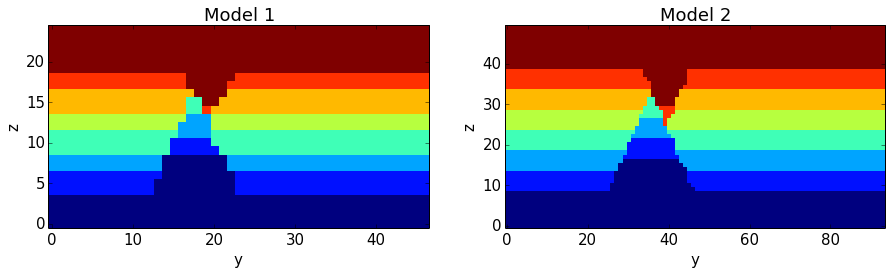
\includegraphics{2-Adjust-input_14_0.png}


\section{(3) Change aspects of geological events}
\label{notebooks/2-Adjust-input:change-aspects-of-geological-events}
Ok, now from some basic settings to the things that we actually want to
change: aspects of the geological history defined in Noddy. This can
happen on two hierarchical levels: on the level of each single event
(i.e. changing parameters relating to one event) and on the level of the
events themselves (i.e. the order of the events).

We will here have a look at the paramteres of the single events:


\chapter{Geological events in pynoddy: organisation and adpatiation}
\label{notebooks/3-Events:geological-events-in-pynoddy-organisation-and-adpatiation}\label{notebooks/3-Events::doc}
We will here describe how the single geological events of a Noddy
history are organised within pynoddy. We will then evaluate in some more
detail how aspects of events can be adapted and their effect evaluated.


\section{Loading events from a Noddy history}
\label{notebooks/3-Events:loading-events-from-a-noddy-history}
In the current set-up of pynoddy, we always start with a pre-defined
Noddy history loaded from a file, and then change aspects of the history
and the single events. The first step is therefore to load the history
file and to extract the single geological events. This is done
automatically as default when loading the history file into the History
object:

\begin{Verbatim}[commandchars=\\\{\}]
\PYG{k+kn}{import} \PYG{n+nn}{sys}\PYG{o}{,} \PYG{n+nn}{os}
\PYG{k+kn}{import} \PYG{n+nn}{matplotlib.pyplot} \PYG{k+kn}{as} \PYG{n+nn}{plt}
\PYG{c}{\PYGZsh{} adjust some settings for matplotlib}
\PYG{k+kn}{from} \PYG{n+nn}{matplotlib} \PYG{k+kn}{import} \PYG{n}{rcParams}
\PYG{c}{\PYGZsh{} print rcParams}
\PYG{n}{rcParams}\PYG{p}{[}\PYG{l+s}{\PYGZsq{}}\PYG{l+s}{font.size}\PYG{l+s}{\PYGZsq{}}\PYG{p}{]} \PYG{o}{=} \PYG{l+m+mi}{15}
\PYG{c}{\PYGZsh{} determine path of repository to set paths corretly below}
\PYG{c}{\PYGZsh{} os.chdir(r\PYGZsq{}/Users/flow/git/pynoddy/docs/notebooks/\PYGZsq{})\PYGZsh{} some basic module imports}
\PYG{n}{repo\PYGZus{}path} \PYG{o}{=} \PYG{n}{os}\PYG{o}{.}\PYG{n}{path}\PYG{o}{.}\PYG{n}{realpath}\PYG{p}{(}\PYG{l+s}{\PYGZsq{}}\PYG{l+s}{../..}\PYG{l+s}{\PYGZsq{}}\PYG{p}{)}

\PYG{k+kn}{import} \PYG{n+nn}{pynoddy}
\end{Verbatim}

\begin{Verbatim}[commandchars=\\\{\}]
\PYG{c}{\PYGZsh{} Change to sandbox directory to store results}
\PYG{n}{os}\PYG{o}{.}\PYG{n}{chdir}\PYG{p}{(}\PYG{n}{os}\PYG{o}{.}\PYG{n}{path}\PYG{o}{.}\PYG{n}{join}\PYG{p}{(}\PYG{n}{repo\PYGZus{}path}\PYG{p}{,} \PYG{l+s}{\PYGZsq{}}\PYG{l+s}{sandbox}\PYG{l+s}{\PYGZsq{}}\PYG{p}{)}\PYG{p}{)}

\PYG{c}{\PYGZsh{} Path to exmaple directory in this repository}
\PYG{n}{example\PYGZus{}directory} \PYG{o}{=} \PYG{n}{os}\PYG{o}{.}\PYG{n}{path}\PYG{o}{.}\PYG{n}{join}\PYG{p}{(}\PYG{n}{repo\PYGZus{}path}\PYG{p}{,}\PYG{l+s}{\PYGZsq{}}\PYG{l+s}{examples}\PYG{l+s}{\PYGZsq{}}\PYG{p}{)}
\PYG{c}{\PYGZsh{} Compute noddy model for history file}
\PYG{n}{history\PYGZus{}file} \PYG{o}{=} \PYG{l+s}{\PYGZsq{}}\PYG{l+s}{simple\PYGZus{}two\PYGZus{}faults.his}\PYG{l+s}{\PYGZsq{}}
\PYG{n}{history} \PYG{o}{=} \PYG{n}{os}\PYG{o}{.}\PYG{n}{path}\PYG{o}{.}\PYG{n}{join}\PYG{p}{(}\PYG{n}{example\PYGZus{}directory}\PYG{p}{,} \PYG{n}{history\PYGZus{}file}\PYG{p}{)}
\PYG{n}{output\PYGZus{}name} \PYG{o}{=} \PYG{l+s}{\PYGZsq{}}\PYG{l+s}{noddy\PYGZus{}out}\PYG{l+s}{\PYGZsq{}}
\PYG{n+nb}{reload}\PYG{p}{(}\PYG{n}{pynoddy}\PYG{o}{.}\PYG{n}{history}\PYG{p}{)}
\PYG{n}{H1} \PYG{o}{=} \PYG{n}{pynoddy}\PYG{o}{.}\PYG{n}{history}\PYG{o}{.}\PYG{n}{NoddyHistory}\PYG{p}{(}\PYG{n}{history}\PYG{p}{)}
\end{Verbatim}

\begin{Verbatim}[commandchars=\\\{\}]
\PYG{l+m+mi}{8}
\end{Verbatim}

Events are stored in the object dictionary ``events'' (who would have
thought), where the key corresponds to the position in the timeline:

\begin{Verbatim}[commandchars=\\\{\}]
\PYG{n}{H1}\PYG{o}{.}\PYG{n}{events}
\end{Verbatim}

\begin{Verbatim}[commandchars=\\\{\}]
\PYGZob{}1: \PYGZlt{}pynoddy.events.Stratigraphy instance at 0x10fc90680\PYGZgt{},
 2: \PYGZlt{}pynoddy.events.Fault instance at 0x10fc90098\PYGZgt{},
 3: \PYGZlt{}pynoddy.events.Fault instance at 0x10fc906c8\PYGZgt{}\PYGZcb{}
\end{Verbatim}

We can see here that three events are defined in the history. Events are
organised as objects themselves, containing all the relevant properties
and information about the events. For example, the second fault event is
defined as:

\begin{Verbatim}[commandchars=\\\{\}]
\PYG{n}{H1}\PYG{o}{.}\PYG{n}{events}\PYG{p}{[}\PYG{l+m+mi}{3}\PYG{p}{]}\PYG{o}{.}\PYG{n}{properties}
\end{Verbatim}

\begin{Verbatim}[commandchars=\\\{\}]
\PYG{p}{\PYGZob{}}\PYG{l+s}{\PYGZsq{}}\PYG{l+s}{Amplitude}\PYG{l+s}{\PYGZsq{}}\PYG{p}{:} \PYG{l+m+mf}{2000.0}\PYG{p}{,}
 \PYG{l+s}{\PYGZsq{}}\PYG{l+s}{Blue}\PYG{l+s}{\PYGZsq{}}\PYG{p}{:} \PYG{l+m+mf}{0.0}\PYG{p}{,}
 \PYG{l+s}{\PYGZsq{}}\PYG{l+s}{Color Name}\PYG{l+s}{\PYGZsq{}}\PYG{p}{:} \PYG{l+s}{\PYGZsq{}}\PYG{l+s}{Custom Colour 5}\PYG{l+s}{\PYGZsq{}}\PYG{p}{,}
 \PYG{l+s}{\PYGZsq{}}\PYG{l+s}{Cyl Index}\PYG{l+s}{\PYGZsq{}}\PYG{p}{:} \PYG{l+m+mf}{0.0}\PYG{p}{,}
 \PYG{l+s}{\PYGZsq{}}\PYG{l+s}{Dip}\PYG{l+s}{\PYGZsq{}}\PYG{p}{:} \PYG{l+m+mf}{60.0}\PYG{p}{,}
 \PYG{l+s}{\PYGZsq{}}\PYG{l+s}{Dip Direction}\PYG{l+s}{\PYGZsq{}}\PYG{p}{:} \PYG{l+m+mf}{270.0}\PYG{p}{,}
 \PYG{l+s}{\PYGZsq{}}\PYG{l+s}{Event \PYGZsh{}3}\PYG{l+s}{\PYGZsq{}}\PYG{p}{:} \PYG{l+s}{\PYGZsq{}}\PYG{l+s}{FAULT}\PYG{l+s}{\PYGZsq{}}\PYG{p}{,}
 \PYG{l+s}{\PYGZsq{}}\PYG{l+s}{Geometry}\PYG{l+s}{\PYGZsq{}}\PYG{p}{:} \PYG{l+s}{\PYGZsq{}}\PYG{l+s}{Translation}\PYG{l+s}{\PYGZsq{}}\PYG{p}{,}
 \PYG{l+s}{\PYGZsq{}}\PYG{l+s}{Green}\PYG{l+s}{\PYGZsq{}}\PYG{p}{:} \PYG{l+m+mf}{0.0}\PYG{p}{,}
 \PYG{l+s}{\PYGZsq{}}\PYG{l+s}{Movement}\PYG{l+s}{\PYGZsq{}}\PYG{p}{:} \PYG{l+s}{\PYGZsq{}}\PYG{l+s}{Hanging Wall}\PYG{l+s}{\PYGZsq{}}\PYG{p}{,}
 \PYG{l+s}{\PYGZsq{}}\PYG{l+s}{Pitch}\PYG{l+s}{\PYGZsq{}}\PYG{p}{:} \PYG{l+m+mf}{90.0}\PYG{p}{,}
 \PYG{l+s}{\PYGZsq{}}\PYG{l+s}{Profile Pitch}\PYG{l+s}{\PYGZsq{}}\PYG{p}{:} \PYG{l+m+mf}{90.0}\PYG{p}{,}
 \PYG{l+s}{\PYGZsq{}}\PYG{l+s}{Radius}\PYG{l+s}{\PYGZsq{}}\PYG{p}{:} \PYG{l+m+mf}{1000.0}\PYG{p}{,}
 \PYG{l+s}{\PYGZsq{}}\PYG{l+s}{Red}\PYG{l+s}{\PYGZsq{}}\PYG{p}{:} \PYG{l+m+mf}{254.0}\PYG{p}{,}
 \PYG{l+s}{\PYGZsq{}}\PYG{l+s}{Rotation}\PYG{l+s}{\PYGZsq{}}\PYG{p}{:} \PYG{l+m+mf}{30.0}\PYG{p}{,}
 \PYG{l+s}{\PYGZsq{}}\PYG{l+s}{Slip}\PYG{l+s}{\PYGZsq{}}\PYG{p}{:} \PYG{l+m+mf}{1000.0}\PYG{p}{,}
 \PYG{l+s}{\PYGZsq{}}\PYG{l+s}{X}\PYG{l+s}{\PYGZsq{}}\PYG{p}{:} \PYG{l+m+mf}{5500.0}\PYG{p}{,}
 \PYG{l+s}{\PYGZsq{}}\PYG{l+s}{XAxis}\PYG{l+s}{\PYGZsq{}}\PYG{p}{:} \PYG{l+m+mf}{2000.0}\PYG{p}{,}
 \PYG{l+s}{\PYGZsq{}}\PYG{l+s}{Y}\PYG{l+s}{\PYGZsq{}}\PYG{p}{:} \PYG{l+m+mf}{7000.0}\PYG{p}{,}
 \PYG{l+s}{\PYGZsq{}}\PYG{l+s}{YAxis}\PYG{l+s}{\PYGZsq{}}\PYG{p}{:} \PYG{l+m+mf}{2000.0}\PYG{p}{,}
 \PYG{l+s}{\PYGZsq{}}\PYG{l+s}{Z}\PYG{l+s}{\PYGZsq{}}\PYG{p}{:} \PYG{l+m+mf}{5000.0}\PYG{p}{,}
 \PYG{l+s}{\PYGZsq{}}\PYG{l+s}{ZAxis}\PYG{l+s}{\PYGZsq{}}\PYG{p}{:} \PYG{l+m+mf}{2000.0}\PYG{p}{\PYGZcb{}}
\end{Verbatim}


\section{Changing aspects of geological events}
\label{notebooks/3-Events:changing-aspects-of-geological-events}
So what we now want to do, of course, is to change aspects of these
events and to evaluate the effect on the resulting geological model.

Changes can be performed directly on the level of the Fault.properties
dictionary:

\begin{Verbatim}[commandchars=\\\{\}]
\PYG{c}{\PYGZsh{} get the original dip of the fault}
\PYG{n}{dip\PYGZus{}ori} \PYG{o}{=} \PYG{n}{H1}\PYG{o}{.}\PYG{n}{events}\PYG{p}{[}\PYG{l+m+mi}{3}\PYG{p}{]}\PYG{o}{.}\PYG{n}{properties}\PYG{p}{[}\PYG{l+s}{\PYGZsq{}}\PYG{l+s}{Dip}\PYG{l+s}{\PYGZsq{}}\PYG{p}{]}
\PYG{c}{\PYGZsh{} add 10 degrees to dip}
\PYG{n}{dip\PYGZus{}new} \PYG{o}{=} \PYG{n}{dip\PYGZus{}ori} \PYG{o}{+} \PYG{l+m+mi}{10}
\PYG{c}{\PYGZsh{} and assign back to properties dictionary:}
\PYG{n}{H1}\PYG{o}{.}\PYG{n}{events}\PYG{p}{[}\PYG{l+m+mi}{3}\PYG{p}{]}\PYG{o}{.}\PYG{n}{properties}\PYG{p}{[}\PYG{l+s}{\PYGZsq{}}\PYG{l+s}{Dip}\PYG{l+s}{\PYGZsq{}}\PYG{p}{]} \PYG{o}{=} \PYG{n}{dip\PYGZus{}new}
\end{Verbatim}

What is left now is to write the model back to a new history file, to
recompute the model, and then visualise the output, as before, to
compare the results:

\begin{Verbatim}[commandchars=\\\{\}]
\PYG{n}{H1}\PYG{o}{.}\PYG{n}{write\PYGZus{}history}\PYG{p}{(}\PYG{n}{new\PYGZus{}history}\PYG{p}{)}
\PYG{n}{pynoddy}\PYG{o}{.}\PYG{n}{compute\PYGZus{}model}\PYG{p}{(}\PYG{n}{new\PYGZus{}history}\PYG{p}{,} \PYG{n}{new\PYGZus{}output}\PYG{p}{)}
\end{Verbatim}

\begin{Verbatim}[commandchars=\\\{\}]
\PYG{n}{H1}\PYG{o}{.}\PYG{n}{all\PYGZus{}events\PYGZus{}end}
\end{Verbatim}

\begin{Verbatim}[commandchars=\\\{\}]
\PYG{l+m+mi}{761}
\end{Verbatim}

\begin{Verbatim}[commandchars=\\\{\}]
n\PYGZus{}lines = 0
for ev in H1.events.values:
    ev.
\end{Verbatim}

\begin{Verbatim}[commandchars=\\\{\}]
  File \PYGZdq{}\PYGZlt{}ipython\PYGZhy{}input\PYGZhy{}96\PYGZhy{}da469714939a\PYGZgt{}\PYGZdq{}, line 3
    ev.
       \PYGZca{}
SyntaxError: invalid syntax
\end{Verbatim}

\begin{Verbatim}[commandchars=\\\{\}]
\PYG{k}{print} \PYG{n}{H1}\PYG{o}{.}\PYG{n}{history\PYGZus{}lines}\PYG{p}{[}\PYG{n}{H1}\PYG{o}{.}\PYG{n}{all\PYGZus{}events\PYGZus{}begin}\PYG{p}{]}
\PYG{k}{print} \PYG{n}{H1}\PYG{o}{.}\PYG{n}{history\PYGZus{}lines}\PYG{p}{[}\PYG{n}{H1}\PYG{o}{.}\PYG{n}{all\PYGZus{}events\PYGZus{}end}\PYG{p}{]}
\end{Verbatim}

\begin{Verbatim}[commandchars=\\\{\}]
Event \PYGZsh{}1    = STRATIGRAPHY

    Name    = Fault1
\end{Verbatim}

\begin{Verbatim}[commandchars=\\\{\}]
\PYG{n}{a} \PYG{o}{=} \PYG{p}{[}\PYG{l+m+mi}{2}\PYG{p}{,}\PYG{l+m+mi}{3}\PYG{p}{]}
\PYG{n}{b} \PYG{o}{=} \PYG{p}{[}\PYG{l+m+mi}{4}\PYG{p}{,}\PYG{l+m+mi}{5}\PYG{p}{]}
\PYG{n}{c} \PYG{o}{=} \PYG{p}{[}\PYG{p}{]}
\PYG{n}{c}\PYG{o}{.}\PYG{n}{append}\PYG{p}{(}\PYG{p}{[}\PYG{n}{a1} \PYG{k}{for} \PYG{n}{a1} \PYG{o+ow}{in} \PYG{n}{a}\PYG{p}{]}\PYG{p}{)}
\PYG{n}{c}\PYG{o}{.}\PYG{n}{append}\PYG{p}{(}\PYG{n}{b}\PYG{p}{[}\PYG{p}{:}\PYG{p}{]}\PYG{p}{)}
\PYG{n}{c}
\end{Verbatim}

\begin{Verbatim}[commandchars=\\\{\}]
\PYG{p}{[}\PYG{p}{[}\PYG{l+m+mi}{2}\PYG{p}{,} \PYG{l+m+mi}{3}\PYG{p}{]}\PYG{p}{,} \PYG{p}{[}\PYG{l+m+mi}{4}\PYG{p}{,} \PYG{l+m+mi}{5}\PYG{p}{]}\PYG{p}{]}
\end{Verbatim}

\begin{Verbatim}[commandchars=\\\{\}]
\PYG{n}{a}\PYG{o}{.}\PYG{n}{pop}\PYG{p}{(}\PYG{p}{)}
\end{Verbatim}

\begin{Verbatim}[commandchars=\\\{\}]
\PYG{l+m+mi}{3}
\end{Verbatim}


\section{Changing the order of geological events}
\label{notebooks/3-Events:changing-the-order-of-geological-events}
The geological history is parameterised as single events in a timeline.
Changing the order of events can be performed with two basic methods:
\begin{enumerate}
\item {} 
Swapping two events with a simple command

\item {} 
Adjusting the entire timeline with a complete remapping of events

\end{enumerate}

The first method is probably the most useful to test how a simple change
in the order of events will effect the final geological model. We will
use it here with our example to test how the model would change if the
timing of the faults is swapped.

The method to swap two geological events is defined on the level of the
history object:

\begin{Verbatim}[commandchars=\\\{\}]
\PYG{n+nb}{reload}\PYG{p}{(}\PYG{n}{pynoddy}\PYG{o}{.}\PYG{n}{history}\PYG{p}{)}
\PYG{n+nb}{reload}\PYG{p}{(}\PYG{n}{pynoddy}\PYG{o}{.}\PYG{n}{events}\PYG{p}{)}
\PYG{n}{H1} \PYG{o}{=} \PYG{n}{pynoddy}\PYG{o}{.}\PYG{n}{history}\PYG{o}{.}\PYG{n}{NoddyHistory}\PYG{p}{(}\PYG{n}{history}\PYG{p}{)}
\end{Verbatim}

\begin{Verbatim}[commandchars=\\\{\}]
\PYG{l+m+mi}{8}
\end{Verbatim}

\begin{Verbatim}[commandchars=\\\{\}]
\PYG{c}{\PYGZsh{} The names of the two fault events defined in the history file are:}
\PYG{k}{print} \PYG{n}{H1}\PYG{o}{.}\PYG{n}{events}\PYG{p}{[}\PYG{l+m+mi}{2}\PYG{p}{]}\PYG{o}{.}\PYG{n}{name}
\PYG{k}{print} \PYG{n}{H1}\PYG{o}{.}\PYG{n}{events}\PYG{p}{[}\PYG{l+m+mi}{3}\PYG{p}{]}\PYG{o}{.}\PYG{n}{name}
\PYG{k}{print} \PYG{n}{H1}\PYG{o}{.}\PYG{n}{events}\PYG{p}{[}\PYG{l+m+mi}{2}\PYG{p}{]}\PYG{o}{.}\PYG{n}{event\PYGZus{}lines}\PYG{p}{[}\PYG{o}{\PYGZhy{}}\PYG{l+m+mi}{4}\PYG{p}{:}\PYG{p}{]}
\PYG{k}{print} \PYG{n}{H1}\PYG{o}{.}\PYG{n}{events}\PYG{p}{[}\PYG{l+m+mi}{3}\PYG{p}{]}\PYG{o}{.}\PYG{n}{event\PYGZus{}lines}\PYG{p}{[}\PYG{o}{\PYGZhy{}}\PYG{l+m+mi}{4}\PYG{p}{:}\PYG{p}{]}
\end{Verbatim}
\begin{alltt}
Fault1
Fault2
{[}'tSurface XDimt= 0.000000rn', `tSurface YDimt= 0.000000rn', `tSurface ZDimt= 0.000000rn', `tNamet= Fault1rn'{]}
{[}'tSurface XDimt= 0.000000rn', `tSurface YDimt= 0.000000rn', `tSurface ZDimt= 0.000000rn', `tNamet= Fault2rn'{]}
\end{alltt}

\begin{Verbatim}[commandchars=\\\{\}]
\PYG{c}{\PYGZsh{} Now: swap the events:}
\PYG{n}{H1}\PYG{o}{.}\PYG{n}{swap\PYGZus{}events}\PYG{p}{(}\PYG{l+m+mi}{2}\PYG{p}{,}\PYG{l+m+mi}{3}\PYG{p}{)}
\end{Verbatim}

\begin{Verbatim}[commandchars=\\\{\}]
\PYG{c}{\PYGZsh{} And let\PYGZsq{}s check if this is correctly relfected in the events order now:}
\PYG{k}{print} \PYG{n}{H1}\PYG{o}{.}\PYG{n}{events}\PYG{p}{[}\PYG{l+m+mi}{2}\PYG{p}{]}\PYG{o}{.}\PYG{n}{name}
\PYG{k}{print} \PYG{n}{H1}\PYG{o}{.}\PYG{n}{events}\PYG{p}{[}\PYG{l+m+mi}{3}\PYG{p}{]}\PYG{o}{.}\PYG{n}{name}
\PYG{k}{print} \PYG{n}{H1}\PYG{o}{.}\PYG{n}{events}\PYG{p}{[}\PYG{l+m+mi}{2}\PYG{p}{]}\PYG{o}{.}\PYG{n}{event\PYGZus{}lines}\PYG{p}{[}\PYG{o}{\PYGZhy{}}\PYG{l+m+mi}{4}\PYG{p}{:}\PYG{p}{]}
\PYG{k}{print} \PYG{n}{H1}\PYG{o}{.}\PYG{n}{events}\PYG{p}{[}\PYG{l+m+mi}{3}\PYG{p}{]}\PYG{o}{.}\PYG{n}{event\PYGZus{}lines}\PYG{p}{[}\PYG{o}{\PYGZhy{}}\PYG{l+m+mi}{4}\PYG{p}{:}\PYG{p}{]}
\end{Verbatim}
\begin{alltt}
Fault1
Fault2
{[}'tSurface XDimt= 0.000000rn', `tSurface YDimt= 0.000000rn', `tSurface ZDimt= 0.000000rn', `tNamet= Fault1rn'{]}
{[}'tSurface XDimt= 0.000000rn', `tSurface YDimt= 0.000000rn', `tSurface ZDimt= 0.000000rn', `tNamet= Fault2rn'{]}
\end{alltt}

Now let's create a new history file and evaluate the effect of the
changed order in a cross section view:

\begin{Verbatim}[commandchars=\\\{\}]
\PYG{n}{new\PYGZus{}history} \PYG{o}{=} \PYG{l+s}{\PYGZdq{}}\PYG{l+s}{faults\PYGZus{}changed\PYGZus{}order.his}\PYG{l+s}{\PYGZdq{}}
\PYG{n}{new\PYGZus{}output} \PYG{o}{=} \PYG{l+s}{\PYGZdq{}}\PYG{l+s}{faults\PYGZus{}out}\PYG{l+s}{\PYGZdq{}}
\PYG{n}{H1}\PYG{o}{.}\PYG{n}{write\PYGZus{}history}\PYG{p}{(}\PYG{n}{new\PYGZus{}history}\PYG{p}{)}
\PYG{n}{pynoddy}\PYG{o}{.}\PYG{n}{compute\PYGZus{}model}\PYG{p}{(}\PYG{n}{new\PYGZus{}history}\PYG{p}{,} \PYG{n}{new\PYGZus{}output}\PYG{p}{)}
\end{Verbatim}

\begin{Verbatim}[commandchars=\\\{\}]
\PYG{c}{\PYGZsh{} Load and compare both models}
\PYG{n}{NO2} \PYG{o}{=} \PYG{n}{pynoddy}\PYG{o}{.}\PYG{n}{NoddyOutput}\PYG{p}{(}\PYG{n}{output\PYGZus{}name}\PYG{p}{)}
\PYG{n}{NO2} \PYG{o}{=} \PYG{n}{pynoddy}\PYG{o}{.}\PYG{n}{NoddyOutput}\PYG{p}{(}\PYG{n}{new\PYGZus{}output}\PYG{p}{)}
\PYG{c}{\PYGZsh{} create basic figure layout}
\PYG{n}{fig} \PYG{o}{=} \PYG{n}{plt}\PYG{o}{.}\PYG{n}{figure}\PYG{p}{(}\PYG{n}{figsize} \PYG{o}{=} \PYG{p}{(}\PYG{l+m+mi}{15}\PYG{p}{,}\PYG{l+m+mi}{5}\PYG{p}{)}\PYG{p}{)}
\PYG{n}{ax1} \PYG{o}{=} \PYG{n}{fig}\PYG{o}{.}\PYG{n}{add\PYGZus{}subplot}\PYG{p}{(}\PYG{l+m+mi}{121}\PYG{p}{)}
\PYG{n}{ax2} \PYG{o}{=} \PYG{n}{fig}\PYG{o}{.}\PYG{n}{add\PYGZus{}subplot}\PYG{p}{(}\PYG{l+m+mi}{122}\PYG{p}{)}
\PYG{n}{NO1}\PYG{o}{.}\PYG{n}{plot\PYGZus{}section}\PYG{p}{(}\PYG{l+s}{\PYGZsq{}}\PYG{l+s}{x}\PYG{l+s}{\PYGZsq{}}\PYG{p}{,} \PYG{n}{ax} \PYG{o}{=} \PYG{n}{ax1}\PYG{p}{,} \PYG{n}{colorbar}\PYG{o}{=}\PYG{n+nb+bp}{False}\PYG{p}{,} \PYG{n}{title}\PYG{o}{=}\PYG{l+s}{\PYGZdq{}}\PYG{l+s}{Model 1}\PYG{l+s}{\PYGZdq{}}\PYG{p}{)}
\PYG{n}{NO2}\PYG{o}{.}\PYG{n}{plot\PYGZus{}section}\PYG{p}{(}\PYG{l+s}{\PYGZsq{}}\PYG{l+s}{x}\PYG{l+s}{\PYGZsq{}}\PYG{p}{,} \PYG{n}{ax} \PYG{o}{=} \PYG{n}{ax2}\PYG{p}{,} \PYG{n}{colorbar}\PYG{o}{=}\PYG{n+nb+bp}{False}\PYG{p}{,} \PYG{n}{title}\PYG{o}{=}\PYG{l+s}{\PYGZdq{}}\PYG{l+s}{Model 2}\PYG{l+s}{\PYGZdq{}}\PYG{p}{)}

\PYG{n}{plt}\PYG{o}{.}\PYG{n}{show}\PYG{p}{(}\PYG{p}{)}
\end{Verbatim}

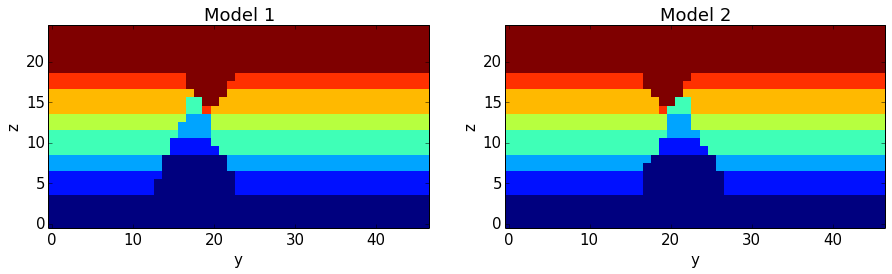
\includegraphics{3-Events_25_0.png}


\chapter{Stochastic events}
\label{notebooks/4-Stochastic-Events::doc}\label{notebooks/4-Stochastic-Events:stochastic-events}
The parameters defining the geological events are, by their very nature,
highly uncertain. In addition to these uncertainties, the kinematic
approach by itself is only a limiting approximation. The picture that we
obtain from the kinematic forword model is therefore a very
overconfident repsresentation of reality - an aspect that (hopefully)
everyone using Noddy is aware of...

In order to respect the vast nature of these uncertainties, we introduce
here an adapted version of the standard geological events defined in
Noddy: the definition of a stochastic event:

A stochastic event is geological event in the Noddy history that has an
uncertainty associated to it in such a way that, recomputing the
geolgoical history will result in a different result each time (note:
the definition is borrowed from the notion of stochastic events in
probabilistic programming, see for example pymc).


\section{Definition of stochastic events}
\label{notebooks/4-Stochastic-Events:definition-of-stochastic-events}
We start, as before, with a pre-defined geological noddy history for
simplicity:


\chapter{pynoddy package}
\label{pynoddy:pynoddy-package}\label{pynoddy::doc}

\section{Submodules}
\label{pynoddy:submodules}

\section{pynoddy.history module}
\label{pynoddy:pynoddy-history-module}\label{pynoddy:module-pynoddy.history}\index{pynoddy.history (module)}
Noddy history file wrapper
Created on 24/03/2014

@author: Florian Wellmann
\index{NoddyHistory (class in pynoddy.history)}

\begin{fulllineitems}
\phantomsection\label{pynoddy:pynoddy.history.NoddyHistory}\pysiglinewithargsret{\strong{class }\code{pynoddy.history.}\bfcode{NoddyHistory}}{\emph{history}}{}
Class container for Noddy history files
\index{change\_cube\_size() (pynoddy.history.NoddyHistory method)}

\begin{fulllineitems}
\phantomsection\label{pynoddy:pynoddy.history.NoddyHistory.change_cube_size}\pysiglinewithargsret{\bfcode{change\_cube\_size}}{\emph{cube\_size}}{}
Change the model cube size (isotropic)
\begin{description}
\item[{\textbf{Arguments}:}] \leavevmode\begin{itemize}
\item {} 
\emph{cube\_size} = float : new model cube size

\end{itemize}

\end{description}

\end{fulllineitems}

\index{determine\_events() (pynoddy.history.NoddyHistory method)}

\begin{fulllineitems}
\phantomsection\label{pynoddy:pynoddy.history.NoddyHistory.determine_events}\pysiglinewithargsret{\bfcode{determine\_events}}{}{}
Determine events and save line numbers

\begin{notice}{note}{Note:}
Parsing of the history file is based on a fixed Noddy output order. 
If this is, for some reason (e.g. in a changed version of Noddy) not the case, then
this parsing might fail!
\end{notice}

\end{fulllineitems}

\index{load\_history() (pynoddy.history.NoddyHistory method)}

\begin{fulllineitems}
\phantomsection\label{pynoddy:pynoddy.history.NoddyHistory.load_history}\pysiglinewithargsret{\bfcode{load\_history}}{\emph{history}}{}
Load Noddy history
\begin{description}
\item[{\textbf{Arguments}:}] \leavevmode\begin{itemize}
\item {} 
\emph{history} = string : Name of Noddy history file

\end{itemize}

\end{description}

\end{fulllineitems}

\index{swap\_events() (pynoddy.history.NoddyHistory method)}

\begin{fulllineitems}
\phantomsection\label{pynoddy:pynoddy.history.NoddyHistory.swap_events}\pysiglinewithargsret{\bfcode{swap\_events}}{\emph{event\_num\_1}, \emph{event\_num\_2}}{}
Swap two geological events in the timeline
\begin{description}
\item[{\textbf{Arguments}:}] \leavevmode\begin{itemize}
\item {} 
\emph{event\_num\_1/2} = int : number of events to be swapped (``order'')

\end{itemize}

\end{description}

\end{fulllineitems}

\index{write\_history() (pynoddy.history.NoddyHistory method)}

\begin{fulllineitems}
\phantomsection\label{pynoddy:pynoddy.history.NoddyHistory.write_history}\pysiglinewithargsret{\bfcode{write\_history}}{\emph{filename}}{}
Write history to new file
\begin{description}
\item[{\textbf{Arguments}:}] \leavevmode\begin{itemize}
\item {} 
\emph{filename} = string : filename of new history file

\end{itemize}

\end{description}

\begin{notice}{hint}{Hint:}
Just love it how easy it is to `write history' with Noddy ;-)
\end{notice}

\end{fulllineitems}


\end{fulllineitems}



\section{pynoddy.output module}
\label{pynoddy:module-pynoddy.output}\label{pynoddy:pynoddy-output-module}\index{pynoddy.output (module)}
Noddy output file analysis
Created on 24/03/2014

@author: Florian Wellmann
\index{NoddyOutput (class in pynoddy.output)}

\begin{fulllineitems}
\phantomsection\label{pynoddy:pynoddy.output.NoddyOutput}\pysiglinewithargsret{\strong{class }\code{pynoddy.output.}\bfcode{NoddyOutput}}{\emph{output\_name}}{}
Class definition for Noddy output analysis
\index{export\_to\_vtk() (pynoddy.output.NoddyOutput method)}

\begin{fulllineitems}
\phantomsection\label{pynoddy:pynoddy.output.NoddyOutput.export_to_vtk}\pysiglinewithargsret{\bfcode{export\_to\_vtk}}{\emph{**kwds}}{}
Export model to VTK

Export the geology blocks to VTK for visualisation of the entire 3-D model in an
external VTK viewer, e.g. Paraview.

..Note:: Requires pyevtk, available for free on: \href{https://github.com/firedrakeproject/firedrake/tree/master/python/evtk}{https://github.com/firedrakeproject/firedrake/tree/master/python/evtk}
\begin{description}
\item[{\textbf{Optional keywords}:}] \leavevmode\begin{itemize}
\item {} 
\emph{vtk\_filename} = string : filename of VTK file (default: output\_name)

\end{itemize}

\end{description}

\end{fulllineitems}

\index{load\_geology() (pynoddy.output.NoddyOutput method)}

\begin{fulllineitems}
\phantomsection\label{pynoddy:pynoddy.output.NoddyOutput.load_geology}\pysiglinewithargsret{\bfcode{load\_geology}}{}{}
Load block geology ids from .g12 output file

\end{fulllineitems}

\index{load\_model\_info() (pynoddy.output.NoddyOutput method)}

\begin{fulllineitems}
\phantomsection\label{pynoddy:pynoddy.output.NoddyOutput.load_model_info}\pysiglinewithargsret{\bfcode{load\_model\_info}}{}{}
Load information about model discretisation from .g00 file

\end{fulllineitems}

\index{plot\_section() (pynoddy.output.NoddyOutput method)}

\begin{fulllineitems}
\phantomsection\label{pynoddy:pynoddy.output.NoddyOutput.plot_section}\pysiglinewithargsret{\bfcode{plot\_section}}{\emph{direction='y'}, \emph{position='center'}, \emph{**kwds}}{}
Create a section block through the model
\begin{description}
\item[{\textbf{Arguments}:}] \leavevmode\begin{itemize}
\item {} 
\emph{direction} = `x', `y', `z' : coordinate direction of section plot (default: `y')

\item {} \begin{description}
\item[{\emph{position} = int or `center'}] \leavevmode{[}cell position of section as integer value{]}
or identifier (default: `center')

\end{description}

\end{itemize}

\item[{\textbf{Optional Keywords}:}] \leavevmode\begin{itemize}
\item {} 
\emph{ax} = matplotlib.axis : append plot to axis (default: create new plot)

\item {} 
\emph{figsize} = (x,y) : matplotlib figsize

\item {} 
\emph{colorbar} = bool : plot colorbar (default: True)

\item {} 
\emph{title} = string : plot title

\item {} 
\emph{savefig} = bool : save figure to file (default: show directly on screen)

\item {} 
\emph{cmap} = matplotlib.cmap : colormap

\item {} 
\emph{fig\_filename} = string : figure filename

\end{itemize}

\end{description}

\end{fulllineitems}

\index{test() (pynoddy.output.NoddyOutput method)}

\begin{fulllineitems}
\phantomsection\label{pynoddy:pynoddy.output.NoddyOutput.test}\pysiglinewithargsret{\bfcode{test}}{}{}
\end{fulllineitems}


\end{fulllineitems}



\section{Module contents}
\label{pynoddy:module-contents}\label{pynoddy:module-pynoddy}\index{pynoddy (module)}
Package initialization file for pynoddy
\index{compute\_model() (in module pynoddy)}

\begin{fulllineitems}
\phantomsection\label{pynoddy:pynoddy.compute_model}\pysiglinewithargsret{\code{pynoddy.}\bfcode{compute\_model}}{\emph{history}, \emph{output\_name}}{}
\end{fulllineitems}



\chapter{Indices and tables}
\label{index:indices-and-tables}\begin{itemize}
\item {} 
\emph{genindex}

\item {} 
\emph{modindex}

\item {} 
\emph{search}

\end{itemize}


\renewcommand{\indexname}{Python Module Index}
\begin{theindex}
\def\bigletter#1{{\Large\sffamily#1}\nopagebreak\vspace{1mm}}
\bigletter{p}
\item {\texttt{pynoddy}}, \pageref{pynoddy:module-pynoddy}
\item {\texttt{pynoddy.history}}, \pageref{pynoddy:module-pynoddy.history}
\item {\texttt{pynoddy.output}}, \pageref{pynoddy:module-pynoddy.output}
\end{theindex}

\renewcommand{\indexname}{Index}
\printindex
\end{document}
